\documentclass[12pt]{article}
\usepackage[a4paper]{geometry}
\usepackage[utf8]{inputenc}
\usepackage{fancyhdr}
\usepackage{lastpage}
\usepackage{graphicx, wrapfig, subcaption, setspace, booktabs}
\usepackage{graphicx}
\usepackage[T1]{fontenc}
\usepackage[font=small, labelfont=bf]{caption}
\usepackage[protrusion=true, expansion=true]{microtype}
\usepackage[english]{babel}
\usepackage{sectsty}
\usepackage{url, lipsum}
\usepackage[T1]{fontenc}
\usepackage{icomma}
\usepackage{siunitx}
\usepackage{ragged2e}
\usepackage{amsmath}
\usepackage{comment}
\usepackage{enumerate}
\usepackage{anysize}


\newcommand{\HRule}[1]{\rule{\linewidth}{#1}}
\onehalfspacing
\setcounter{tocdepth}{5}
\setcounter{secnumdepth}{5}

\begin{document}

\begin{titlepage}

\title{ \normalsize 
        \begin{center}
        
\includegraphics[height=6cm]{logo.png}
        \end{center}
        \LARGE \textsc{\textbf{Universidad De Sonora}} \\ \bigskip
		\Large División de Ciencias Exactas y Naturales \\
        Licenciatura en Física \\ \bigskip
        \bigskip
        Física Computacional I
		\\ [0.1cm]  
		\HRule{2pt} \\
		\Large \textbf{{Evaluación 1}} \\
        \textit{\textbf{"Análisis de las Mareas y Salinidad en el Manglar El Sargento"}}
		\HRule{2pt} \\
		\normalsize \vspace*{0.001\baselineskip}}
        
\date{\bigskip \Large Hermosillo, Sonora  \hspace*{\fill}  Marzo 8 de 2018}

        
\author{
		\Large\textbf{ Michelle Contreras Cossio} \\ \bigskip
        \\ \bigskip
       \Large Profr. Carlos Lizárraga Celaya}
       \end{titlepage}
       \maketitle
       

\newpage
\pagestyle{plain}

\section{Introducción}

Esta es la primera evaluación que se aplica para la materia de Física Computacional; en este documento se presenta tanto el procedimiento realizado, como los resultados.\\

Se utilizan datos reales de la estación de monitoreo de variables atmosféricas en el Manglar "El Sargento", una bahía costera frente a la parte norte de la Isla del Tiburón; las variables con las que se trabajó en la evaluación fueron Nivel del Agua y Salinidad. \\

El objetivo de esta evaluación es dar constancia de lo aprendido en las cinco actividades ya realizadas, haciendo un análisis y lectura de datos pertinentes, para poder graficar y comparar algunas variables como Temperatura, Salinidad, Nivel del agua. Para ello, se hizo uso de pandas en jupyter y de bibliotecas como matplotlib o seaborn. 

\section{Descripción de los conceptos físicos:  Salinidad y Nivel del Agua}

Como se mencionó, las variables de interés en este caso son la salinidad y el nivel del agua, a continuación se definen:\\

La salinidad es el contenido de sales minerales disueltas en un cuerpo de agua. Dicho de otra manera, es válida la expresión salinidad para referirse al contenido salino en suelos o en agua.\\

El nivel del agua, por su parte, es la altura de las aguas del mar cuando está en calma, que sirve de referencia para medir la altura o la profundidad de una montaña, un punto geográfico, etc.

\section{Descripción de la estructura de los archivos}

Los archivos mencionados en esta sección fueron proporcionados por el maestro para realizar la evaluación, descargados del portal de la materia. 

El archivo "sargento-201117.csv", contiene los datos del nivel del mar. Primeramente, su nombre fue cambiaro a " sargento\_201117.csv", para permitir su lectura en pandas. Este archivo de datos, cuenta con 5 columnas: la primera indica el número del dato, la segunda fecha y hora, la tercera la presión en kPa, la cuarta la temperatura en grados centígrados y la quinta el nivel del agua en metros; las columnas se encuentran separadas por comas. Este archivo cuenta con 2395 datos, proporciona datos de cada 15 minutos, empezando el 26 de Octubre del 2017 a las 13 horas y terminando el 20 de Noviembre del 2017 a las 11:30 horas. Un segmento del archivo:

\begin{verbatim}
"Plot Title: sargento-salinidad"
"#","Date Time, GMT-07:00", "Cond High Rng, ?S/cm","Temp, C", "Specific 
Conductance, ?S/cm","Salinity, ppt"
1,10/26/2017 12:45:00,54525.5,25.21,54301.2,35.9195
2,10/26/2017 13:00:00,54525.5,24.91,54622.1,36.1588
3,10/26/2017 13:15:00,54525.5,24.82,54719.0,36.2311
4,10/26/2017 13:30:00,54525.5,24.76,54783.8,36.2794
5,10/26/2017 13:45:00,54525.5,24.75,54794.6,36.2875
\end{verbatim}

El archivo "salinidad\_sargento-201117.csv", contiene los datos de la salinidad, de igual manera sufrió un cambio de nombre, por la misma razón, a "salinidad\_sargento\_201117.csv". Este archivo cuenta con 6 columnas: número del dato, fecha y hora, conductancia en S/cm, temperatura en grados centígrados, conductancia específica en S/cm y salinidad en ppt. El archivo cuenta, de igual manera, con 2395 datos, sin embargo empieza y termina 15 minutos antes que el anterior, por lo que hay un pequeño desfase. A continuación se muestra un segmento del archivo:

\begin{verbatim}
"Plot Title: sargento-salinidad"
"#","Date Time, GMT-07:00","Cond High Rng, ?S/cm","Temp, C", "Specific 
Conductance, ?S/cm","Salinity, ppt"
1,10/26/2017 12:45:00,54525.5,25.21,54301.2,35.9195
2,10/26/2017 13:00:00,54525.5,24.91,54622.1,36.1588
3,10/26/2017 13:15:00,54525.5,24.82,54719.0,36.2311
4,10/26/2017 13:30:00,54525.5,24.76,54783.8,36.2794
5,10/26/2017 13:45:00,54525.5,24.75,54794.6,36.2875
\end{verbatim}

\clearpage

\section{Análisis de datos utilizando Pandas}

En esta sección se muestra el procedimiento que se realizó al momento de trabajar con los archivos de datos, para poder crear las gráficas: 

\begin{enumerate}
\item Como se mencionó en la sección anterior, se descargaron los archivos de la página y el único cambio que se les hizo fue el nombre, para poder leerlos con pandas. 
\item Se inicializó Jupyter en la carpeta creada de la Evaluacion1, misma donde se encuentran los archivos descargados. Creando un archivo nuevo "Evaluacion1.ipynb". 
\item Se descargaron las bibliotecas necesarias: pandas, numpy, matplotlib y datetime. 
\begin{figure}[h!]
  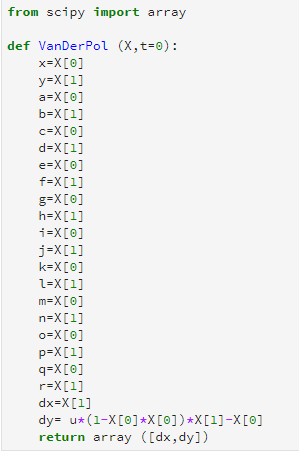
\includegraphics[width=7cm]{1.png}
  \centering
  \label{fig:1}
\end{figure}

\item Se procedió a leer los archivos asignándolos a su data frame correspondiente. Se tomó en cuenta que el archivo con la información de salinidad (df2) debía comenzar un renglón después, para que ambos contaran con datos a partir de las 13:00:00 del 26 de Octubre. Se les dio nombre a las columnas.
\begin{figure}[h!]
  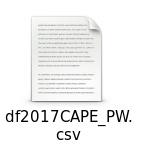
\includegraphics[width=15cm]{2.png}
  \centering
  \label{fig:2}
\end{figure}
\item Con el fin de que ambos dataframes terminaran a las 11:15:00 del 20 de Noviembre, se eliminó el último renglón del data frame con la información del nivel del agua (df1). Y se borró la columna del número de dato de ambos, ya que aprovecharemos el índice para esto.
\begin{figure}[h!]
  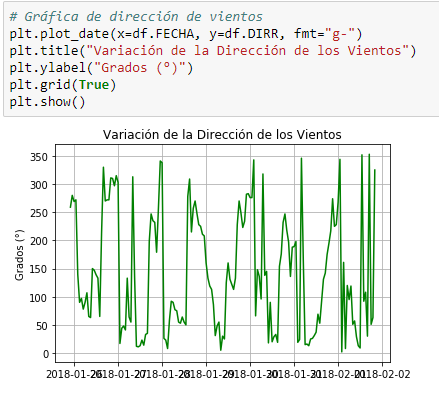
\includegraphics[width=15cm]{3.png}
  \centering
  \label{fig:3}
\end{figure}
\item Se convirtieron las columnas de fecha en formato de fecha y se creó una nueva columna de mes, que nos indica el número del mes, para poder utilizarla posteriormente. 
\begin{figure}[h!]
  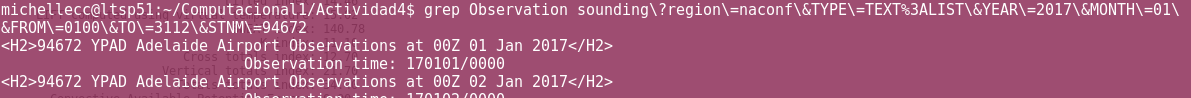
\includegraphics[width=12cm]{4.png}
  \centering
  \label{fig:4}
\end{figure}\\
\\
\item Se reinició el índice de número de dato, para que el de ambos archivos fuera idéntico. Y se verificó que todo haya funcionado utilizando las funciones head y dtypes.
\begin{figure}[h!]
  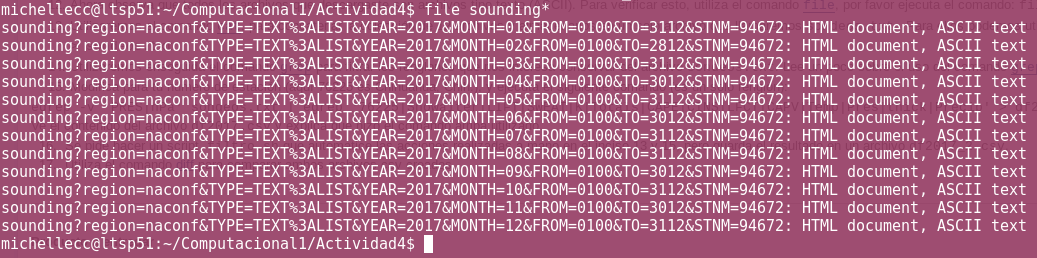
\includegraphics[width=8cm]{5.png}
  \centering
  \label{fig:5}
\end{figure}
\begin{figure}[h!]
  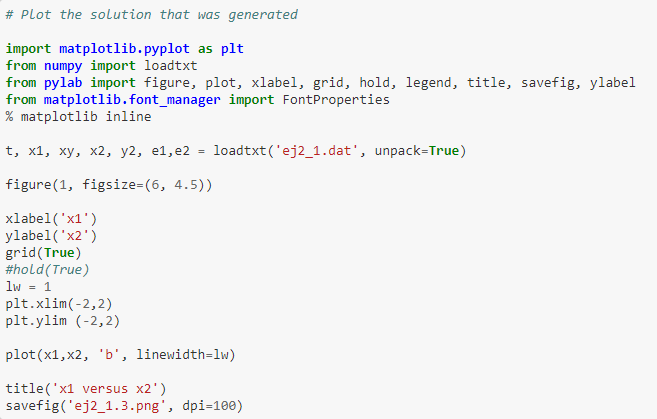
\includegraphics[width=5cm]{6.png}
  \centering
  \label{fig:6}
\end{figure}
\item Comenzando con las gráficas, las primeras fueron los boxplots, las variables WaterLevel, Salinity y Temp fueron graficadas para visualizar su variabilidad en los datos que se tienen de los meses Octubre y Noviembre, para ello se utilizó la columna de mes sobre el eje x. El siguiente segmento de código muestra un ejemplo de como se realizó el boxplot de WaterLevel, las demás se realizaron de manera análoga: 
\begin{figure}[h!]
  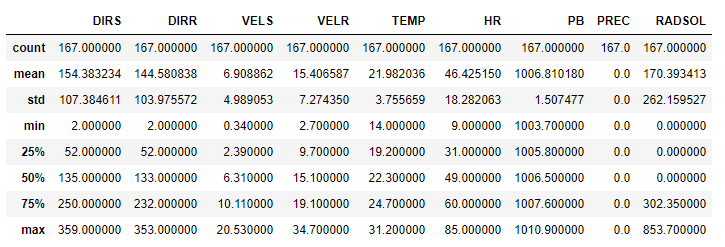
\includegraphics[width=8.5cm]{7.png}
  \centering
  \label{fig:7}
\end{figure}
\item Se utilizó la función describe para poder tener el dato exacto sobre los cuartiles.
\item Posteriormente se realizaron los diagramas de Pearson. El primero pide ver la relación entre el nivel del mar y la salinidad. Para ello se creó un nuevo data frame (df3), que contuviera a estas dos variables, ya que pertenecían al df1 y df2, respectivamente. 
\begin{figure}[h!]
  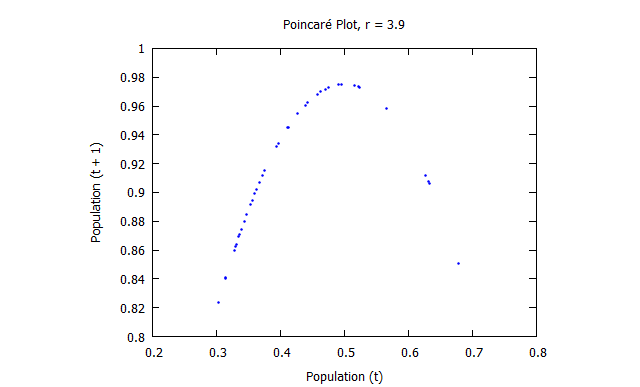
\includegraphics[width=9cm]{8.png}
  \centering
  \label{fig:8}
\end{figure}
\item Una vez que se tuvieron ambas variables juntas, se graficó el Pearson que relacionara ambas. 
\begin{figure}[h!]
  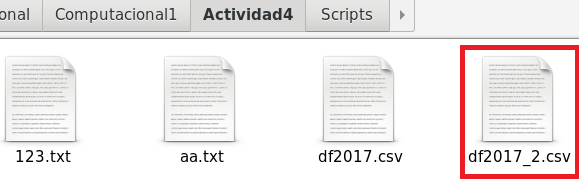
\includegraphics[width=13cm]{9.png}
  \centering
  \label{fig:9}
\end{figure}
\item Para los siguientes dos Pearson no hubo necesidad de crear nuevos data frame, ya que las variables necesarias pertenecían ya a uno mismo. El segundo Pearson fue de nivel de agua y temperatura y el tercero de salinidad y temperatura y se realizaron de manera anáologa al paso anterior.
\item Las siguientes gráficas fueron de las variables nivel del agua, salinidad y temperatura, cada una en función del tiempo, para ello se utilizó la columna de fecha sobre el eje x. A continuación se muestra el código para realizar la del nivel del agua, las otras dos se realizaron de manera análoga: 
\begin{figure}[h!]
  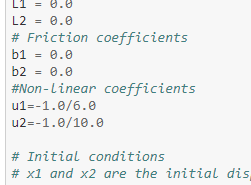
\includegraphics[width=9cm]{10.png}
  \centering
  \label{fig:10}
\end{figure}
\item A continuación, se crearon dos gráficas con doble eje y, uno en la izquierda y uno en la derecha, ya que tienen distinta escala o graduación, en la primera, el eje de la izquierda correspondía a la salinidad y el de la derecha al nivel del agua; en la segunda el nivel del agua y la temperatura, respectivamente. Ambas en función del tiempo, tomando al eje x como la fecha. Se muestra el código para la gráfica Salinidad-Nivel del agua:
\clearpage
\begin{figure}[h!]
  
\includegraphics[width=8cm]{11.png}
  \centering
  \label{fig:11}
\end{figure}
\item Finalmente, las mismas gráficas realizadas en el punto anterior, se volvieron a crear pero limitando las fechas del eje x, en ambos casos de limito del 1ro de Noviembre del 2017 a las 00:00:00 hasta el 5 de Noviembre a las 23:45:00.  Se muestra el código para la gráfica Salinidad-Nivel del agua:
\begin{figure}[h!]
  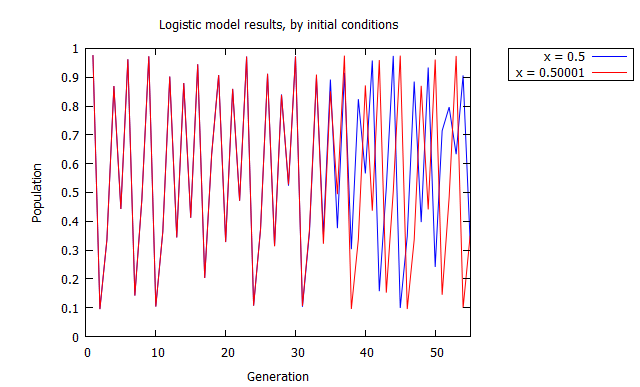
\includegraphics[width=12cm]{12.png}
  \centering
  \label{fig:12}
\end{figure}
\end{enumerate}

\clearpage
\section{Resultados del análisis}

Como bien se mencionó en la sección anterior, el fruto que tuvo este análisis de datos fueron diversas gráficas, a continuación mostradas y discutidas: 
\subsection{Boxplots}

\begin{itemize}
\item \textbf{Nivel del agua:}
\begin{figure}[h!]
  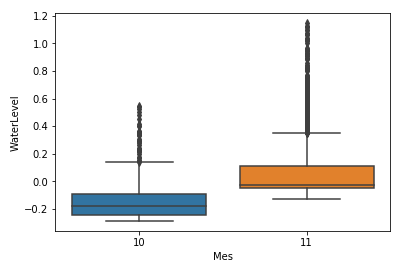
\includegraphics[width=10cm]{g1.png}
  \centering
  \label{fig:g1}
\end{figure}

Se puede observar que la media de nivel del agua de octubre a noviembre aumentó aproximadamente 20 cm. En octubre se encontraba en -.2m y en noviembre alrededor de los 0 m. Ambas tienen una distribución bastante pequeña, se puede observar que el nivel del agua con aumenta de manera considerable, únicamente centímetros. 


\item\textbf{Salinidad:}

\begin{figure}[h!]
  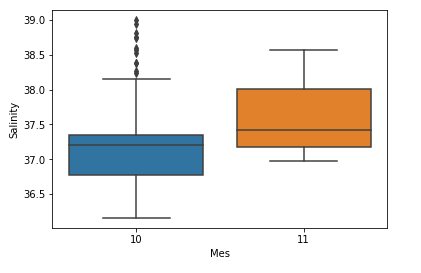
\includegraphics[width=10cm]{g2.png}
  \centering
  \label{fig:g2}
\end{figure}

En este diagrama de caja se observa que aunque las cajas de octubre y noviembre se encuentran algo separadas, la media sigue apareciendo casi en el mismo valor, entre 37 y 37.5.

\item \textbf{Temperatura:}

\begin{figure}[h!]
  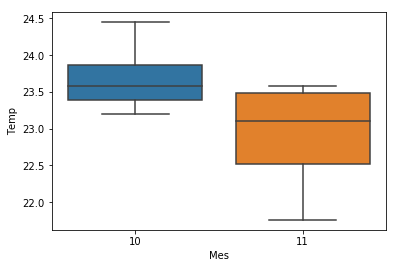
\includegraphics[width=10cm]{g3.png}
  \centering
  \label{fig:g3}
\end{figure}

Este diagrama, al igual que los anteriores, no muestra un cambio bastante considerable de octubre a noviembre, a pesar de que si lo hay, lo que se puede observar es que las temperaturas están bastante fijas entre un rango total de 22 a 24.5$^{\circ}$C. 

\item \textbf{Describes:}

Estos permiten ver un análisis completo de los datos. Sin embargo, no dan la información de donde se encuentran los cuartiles, máximos, mínimos y mediana, necesarias, ya que los datos posteriormente se clasifican por el mes.

\begin{figure}[h!]
  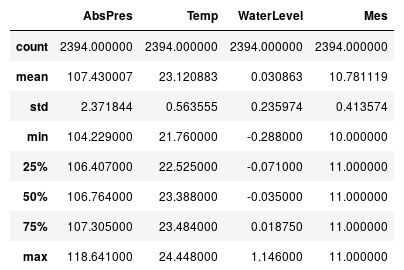
\includegraphics[width=9.5cm]{desc1.png}
  \centering
  \label{fig:d1}
\end{figure}

\begin{figure}[h!]
  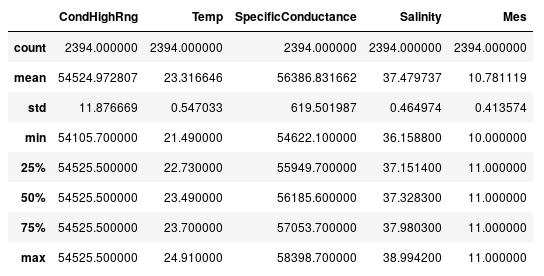
\includegraphics[width=12cm]{desc2.png}
  \centering
  \label{fig:d2}
\end{figure}

\end{itemize}


\subsection{Diagramas de Pearson}

\begin{itemize}
\item \textbf{Salinidad-Nivel del agua:}

\begin{figure}[h!]
  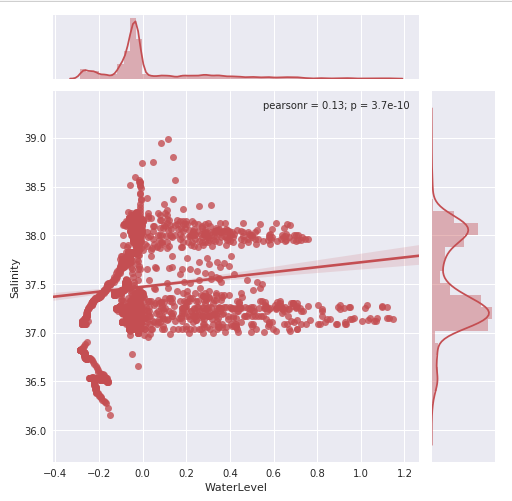
\includegraphics[width=10cm]{g4.png}
  \centering
  \label{fig:g4}
\end{figure}

Con esta gráfica podemos observar que si existe una correlación lineal entre la salinidad y el nivel del agua, aunque no muy fuerte, el pearson=0.13. Se observa que la distribución de la salinidad cuenta con dos picos, mientras que la del nivel del agua con uno. 

\item\textbf{Temperatura-Nivel del agua:}

\begin{figure}[h!]
  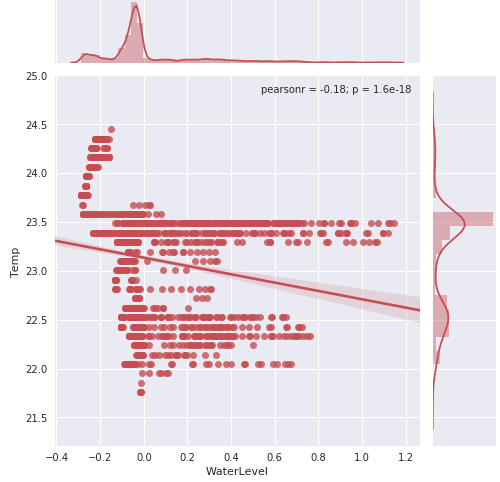
\includegraphics[width=10.5cm]{g5.png}
  \centering
  \label{fig:g5}
\end{figure}

La relación que existe entre estas dos variables es negativa y tampoco es muy grande, aunque existe, ya que el pearson es diferente de 0 y es igual a -0.18

\item \textbf{Temperatura-Salinidad:}

\begin{figure}[h!]
  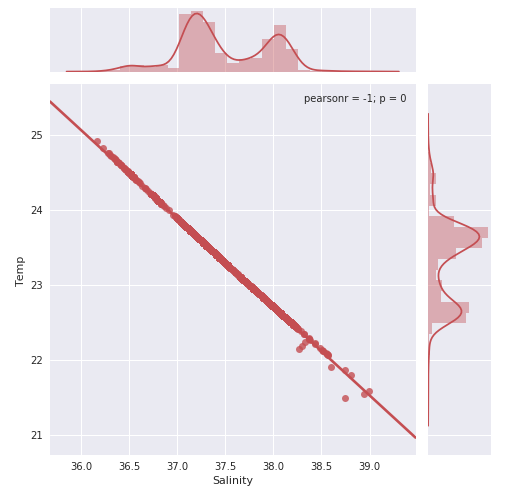
\includegraphics[width=10.5cm]{g6.png}
  \centering
  \label{fig:g6}
\end{figure}

Estas dos variables se encuentran perfectamente correlacionadas negativamente, el pearson es igual a -1, se puede observar que ambas tienen los mismos picos, sus distribuciones, como es de esperarse, son bastante similares. 

\end{itemize}

\subsection{Gráficas en función del tiempo}

\begin{itemize}
\item \textbf{Nivel del agua:}

\begin{figure}[h!]
  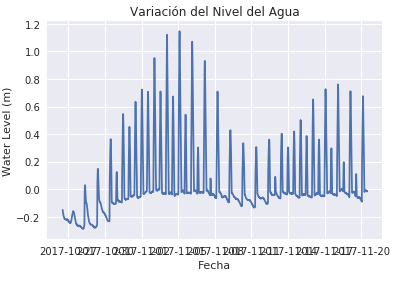
\includegraphics[width=10.5cm]{g7.png}
  \centering
  \label{fig:g7}
\end{figure}

El nivel del agua, conforme el tiempo, empezó a aumentar a principios de noviembre, pero posteriormente disminuyó, para volver a incrementar, teniendo con esto una distribución con dos picos. 

\item\textbf{Salinidad:}
\begin{figure}[h!]
  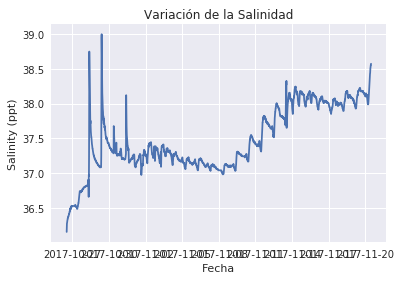
\includegraphics[width=10.5cm]{g8.png}
  \centering
  \label{fig:g8}
\end{figure}

La salinidad, de manera general y aunque cuenta con dos picos a principios de noviembre, fue aumentanto, conforme el tiempo iba pasando. 

\item \textbf{Temperatura:}

\begin{figure}[h!]
  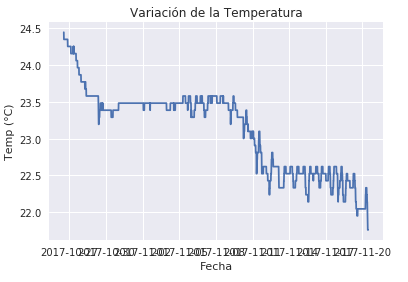
\includegraphics[width=10.5cm]{g9.png}
  \centering
  \label{fig:g9}
\end{figure}

Como era de esperarse, la temperatura fue disminuyendo al paso del tiempo, esto debido a que se acercó el invierno.

\end{itemize}

\subsection{Gráficas de doble eje vertical}

\begin{itemize}
\item \textbf{Salinidad-Nivel del agua:}
\begin{figure}[h!]
  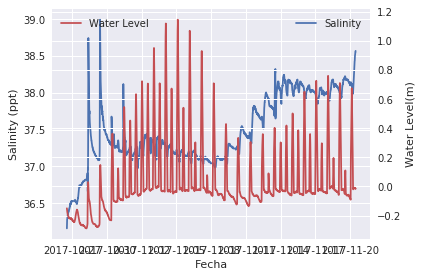
\includegraphics[width=11cm]{g10.png}
  \centering
  \label{fig:g10}
\end{figure}

En esta gráfica se puede comparar la distribución que tienen la salinidad y el nivel del mar en función del tiempo. Se puede ver que las distribuciones no son precisamente parecidas, aunque como se vió con el diagrama de Pearson, podría existir una relación entre ambas. 

\item\textbf{Temperatura-Nivel del agua:}

\begin{figure}[h!]
  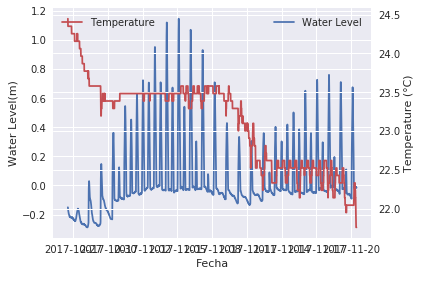
\includegraphics[width=11cm]{g11.png}
  \centering
  \label{fig:g11}
\end{figure}

En esta gráfica se puede comparar la distribución que tienen la temperatura y el nivel del mar en función del tiempo. A simple vista, no se puede observar una dependencia o relación entre ambas, aunque por el diagrama de Pearson, no se puede descartar la existencia de una. 

\end{itemize}

\subsection{Gráficas de doble eje vertical en 5 días}

\begin{itemize}
\item \textbf{Salinidad-Nivel del agua:}

\begin{figure}[h!]
  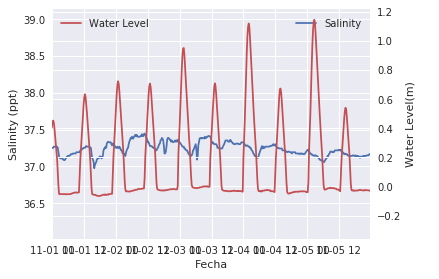
\includegraphics[width=12cm]{g12.png}
  \centering
  \label{fig:g12}
\end{figure}

Con esta gráfica, tomando datos de únicamente 5 días, se puede observar que mientras el nivel del mar aumenta y tiene picos cada día, aproximadamente a las mismas horas, la salinidad parece mantenerse casi constante alrededor de los 37 ppt.

En mi opinión no se observa una dependencia entre ambas, ya que mientras el nivel del mar tiene un comportamiento, casi periódico a lo largo de un día, la salinidad permanece alrededor de una constante, no se ve que el cambio de una afecte a la otra. 

\item\textbf{Temperatura-Nivel del agua:}

\begin{figure}[h!]
  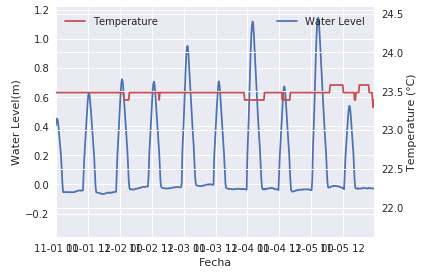
\includegraphics[width=11cm]{g13.png}
  \centering
  \label{fig:g13}
\end{figure}

Al igual que la gráfica pasada, el nivel del mar aumenta y disminuye considerablemente en un mismo día, mientras que la temperatura es casi constante, alrededor de los 23.5$^{\circ}$C.

De igual manera, el nivel del mar tiene un comportamiento que se repite en un mismo día donde a ciertas horas aumenta y a ciertas horas disminuye, mientras que la temperatura parece permanecer constante independientemente de que el nivel del agua cambie. 

\end{itemize}

\clearpage
\section{Conclusiones}

Por último y para concluir, podría agregar que la única relación que vi bastante evidente fue la de la temperatura y la salinidad, a medida que la temperatura disminuye, la salinidad aumenta, y viceversa. La demás relaciones de dependencia no las podría defender como ciertas, a pesar del índice de pearson diferente de cero. \\

Además, como conclusión sobre el examen, me pareció bastante entretenido, aunque un poco largo e imposible de hacer en dos horas, si fue algo agotador, pero valió la pena porque en este me di cuenta de lo mucho que he aprendido y de la facilidad que adquirí para resolver los problemas con los que me encontraba utilizando tutoriales de internet, cosa que se que complicaba al entender la sintaxis con la que se trabajaba. Me gustó y el contenido fue adecuado a lo visto en las actividades anteriores.

\section{Bibliografía}
\begin{itemize}
\item Nivel del mar (2018). Consultado: 8 de Marzo del 2018, de Wikipedia. Sitio web: https://es.wikipedia.org/wiki/Nivel\_del\_mar
\item Salinidad (2018). Consultado: 8 de Marzo del 2018, de Wikipedia. Sitio web:\\ https://es.wikipedia.org/wiki/Salinidad
\end{itemize}





\end{document}